\documentclass[11pt]{exam}

\usepackage[utf8]{inputenc}
\usepackage{hyperref}
\usepackage[spanish]{babel}
\usepackage{graphicx}
\usepackage{listings}
\usepackage[table,xcdraw]{xcolor}

\definecolor{codegreen}{rgb}{0,0.6,0}
\definecolor{codegray}{rgb}{0.5,0.5,0.5}
\definecolor{codepurple}{rgb}{0.58,0,0.82}
\definecolor{backcolour}{rgb}{0.95,0.95,0.92}

\lstdefinestyle{mystyle}{
	backgroundcolor=\color{backcolour},   
	commentstyle=\color{codegreen},
	keywordstyle=\color{magenta},
	%numberstyle=\tiny\color{codegray},
	stringstyle=\color{codepurple},
	basicstyle=\ttfamily\footnotesize,
	breakatwhitespace=false,         
	breaklines=true,                 
	captionpos=b,                    
	keepspaces=true,                 
	%numbers=left,                    
	%numbersep=5pt,                  
	showspaces=false,                
	showstringspaces=false,
	showtabs=false,                  
	tabsize=2
}

\lstset{style=mystyle}

\title{Práctica 1}
\author{Laura Rodríguez Navas \\ rodrigueznavas@posgrado.uimp.es}
\date{{\selectlanguage{spanish}\today} }

\pagestyle{plain}

\begin{document}
	
\maketitle

\section*{Ejercicio 1}

\begin{enumerate}
	\item Descargar el código fuente para esta práctica, \textit{softpractica1.zip}, de la página web de la asignatura.
	\item Descomprimir el fichero anterior.
	\item Abrir un terminal o consola de comandos y entrar dentro de la carpeta \textit{softpractica1}.
	\item Para empezar vamos a ejecutar GridWorld en el modo de control manual, usando el comando \textit{python gridworld.py -m -n 0}, que utiliza las teclas de flecha.	
	\item El objetivo es lograr llegar lo antes posible a la celda etiquetada con un 1, evitando caer en la celda con un -1.
\end{enumerate}

\begin{figure}[h]
	\centering
	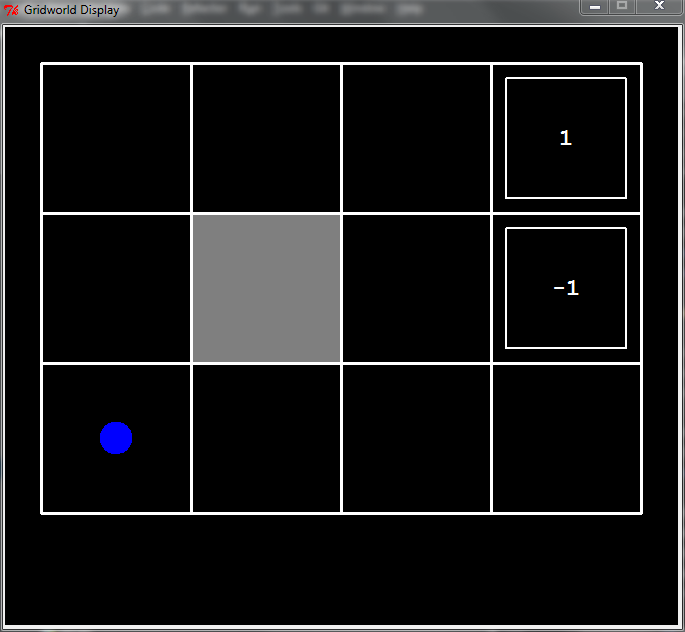
\includegraphics[scale=0.5]{image_1}
	\caption{Interfaz del dominio GridWorld en el modo de control manual.}
	\label{image_1}
\end{figure}

\subsection*{Preguntas}

\begin{questions}
	
% Pregunta 1
{ \question ¿Cuántas celdas/estados aparecen en el tablero? ¿Cuántas acciones puede ejecutar el agente? Si quisieras resolver el juego mediante aprendizaje por refuerzo, ¿cómo lo harías? 
}

En el tablero aparecen 11 celdas/estado y el agente puede ejecutar 4 acciones: arriba (\textit{north}), abajo (\textit{south}), izquierda (\textit{west}) y derecha (\textit{east}).

Para resolver el juego usaremos el algoritmo \href{https://en.wikipedia.org/wiki/Q-learning}{Q-learning} con el objetivo de que el agente llegue lo antes posible a la celda etiquetada con un 1 (estado \textit{done}), evitando caer en la celda con un -1 (estado \textit{exit}). A medida que el agente se mueve por el laberinto, pierde salud gradualmente, por lo que tiene que moverse con un propósito.

La clave del algoritmo Q-learning será la construcción de su tabla \textit{Q}, que es una matriz donde tendremos las recompensas que obtendrá el agente para cada acción y en cada estado, es decir, los valores $Q(s,a)$. El algoritmo hará que el agente vaya tomando decisiones y a cada decisión actualizará uno de los valores $Q(s,a)$ de la tabla \textit{Q}. A la hora de tomar las decisiones el algoritmo usa la estrategia \textit{$\epsilon$}-greedy. Esta estrategia consiste en que todas las acciones sean tomadas buscando el valor máximo de $Q(s,a)$ pero existiendo una probabilidad pequeña \textit{$\epsilon$}, de tomar una decisión aleatoria para que el agente explore todo el espacio de soluciones. Para la actualización de la tabla \textit{Q} e ir completándola, cada decisión tomada por el agente se evaluará por la siguiente expresión:

\begin{equation}
	Q^*(s_{t}, a_{t}) \leftarrow (1-\alpha) \; Q(s_{t}, a_{t}) + \alpha_{t} \; [r_{s_{t}, a_{t}} + \gamma \; max_{a} \; Q(s_{t + 1}, a)]
\end{equation}

En esta expresión $Q(s_{t}, a_{t})$ es el valor de la tabla \textit{Q} del estado $s_{t}$ y la acción $ a_{t}$. $Q^*(s_{t}, a_{t})$ será el nuevo valor de la tabla \textit{Q} para dicho estado y acción. El valor $\gamma$ es el \href{https://en.wikipedia.org/wiki/Learning_rate}{\textit{learning rate}}, que puede tomar valores entre 0 y 1. Finalmente $r_{s_{t}, a_{t}}$, determina la recompensa inmediata asociada a la acción tomada y es el \href{https://en.wikipedia.org/wiki/Discounting#Discount_factor}{\textit{discount factor}} que también puede tomar valores entre 0 y 1.

% Pregunta 2
{ \question Abrir el fichero \textit{qlearningAgents.py} y buscar la clase \textit{QLearningAgent}. Describir los métodos que aparecen en ella.
}

Los métodos que aparecen en la clase \textit{QLearningAgent} son:

\begin{itemize}
	\item \textbf{\_\_init\_\_}: Inicializa la \textit{Q-Table} a partir del fichero \textit{qtable.txt}, es decir, la \textit{Q-Table} se inicializa a cero.
	
	\item \textbf{readQtable}: Lee la \textit{Q-Table} del fichero \textit{qtable.txt}.
	
	\item \textbf{writeQtable}: Escribe la \textit{Q-Table} en el fichero \textit{qtable.txt}.
	
	\item \textbf{\_\_del\_\_}: Llama al método \textit{writeQtable} que escribe el resultado final de la \textit{Q-Table} en el fichero \textit{qtable.txt}.
	
	\item \textbf{computePosition}: Calcula la fila de la \textit{Q-Table} para un estado dado.
	
	\item \textbf{getQValue}: Devuelve el valor $Q(s,a)$ para un estado y una acción dados. De lo contrario, devuelve 0.0, si nunca hemos visto el estado o el valor del nodo $Q$.
	
	\item \textbf{computeValueFromQValues}: Devuelve el valor máximo de $Q(s,a)$ para un estado dado. Este valor se encuentra por encima de las acciones válidas. Si no hay acciones válidas, como en el caso del estado \textit{exit}, devuelve 0.0.
	
	\item \textbf{computeActionFromQValues}: Calcula la mejor acción a realizar para un estado dado. Si no hay acciones válidas, como en el caso del estado \textit{exit}, devuelve \textit{None}.
	
	\item \textbf{getAction}: Calcula la acción a realizar para un estado dado. En caso contrario, con probabilidad \textit{self.epsilon}, elige una acción aleatoria y la mejor acción política. Si no hay acciones válidas, como en el caso del estado \textit{exit}, elige \textit{None} como acción.
	
	\item \textbf{update}: Actualiza la \textit{Q-Table}. El método para un acción dada, observa una recompensa, introduce un estado nuevo (que depende del estado anterior y de la acción dada), y actualiza el valor $Q(s,a)$. 
	
	Si el nuevo estado introducido es el estado \textit{exit}, se sigue la regla:
	
	\begin{center}
		$Q(state,action) <- (1-self.alpha) * Q(state,action) + self.alpha * (reward + 0)$
	\end{center}

	De lo contrario, si el nuevo estado introducido no es el estado \textit{exit}, se sigue la regla:
	
	\begin{center}
		$Q(state,action) <- (1-self.alpha) * Q(state,action) + self.alpha * (reward + self.discount * max a' Q(nextState, a'))$
	\end{center}
	
	\item \textbf{getPolicy}: Devuelve la mejor acción de la \textit{Q-Table} para un estado dado.
	
	\item \textbf{getValue}: Devuelve el valor $Q(s,a)$ más alto para un estado dado.
		
\end{itemize}

% Pregunta 3
{ \question Ejecuta ahora el agente anterior con: \textit{python gridworld.py -a q -k 100 -n 0}.}

A diferencia de la primera ejecución, en esta ejecución le indicamos el tipo de agente, que en este caso es q, y el número de movimientos \href{https://en.wikipedia.org/wiki/Markov_decision_process}{MDP} a realizar, que en este caso son 100.

\begin{figure}[h]
	\centering
	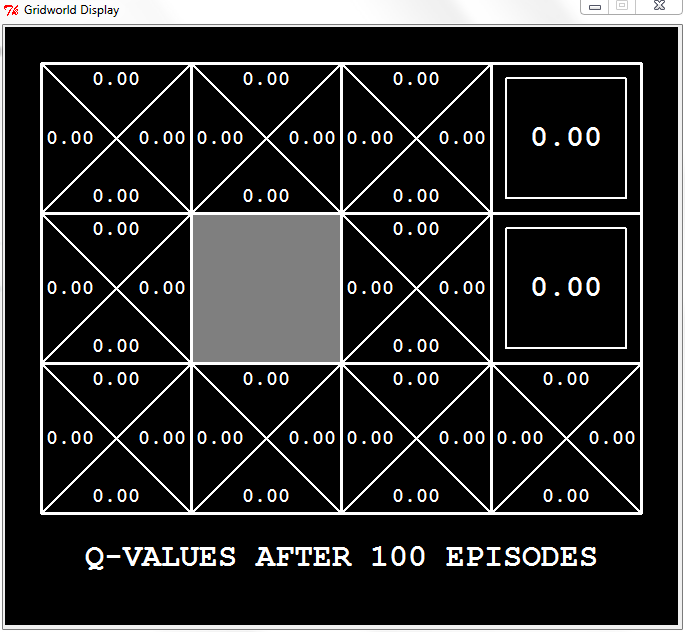
\includegraphics[scale=0.5]{image_2}
	\caption{Interfaz del dominio GridWorld usando \textit{python gridworld.py -a q -k 100 -n 0}.}
	\label{image_2}
\end{figure}

% Pregunta 4
{ \question ¿Qué información se muestra en el laberinto? ¿Qué aparece por terminal cuando se realizan los movimientos en el laberinto? 
}

Si observamos la Figura \ref{image_2}, vemos que la información que se muestra en el laberinto son los valores de $Q(s,a)$ después de realizarse 100 movimientos. 

\newpage

En la terminal cuando se realizan los movimientos en el laberinto, vemos que aparecen los siguientes valores por cada movimiento:

\begin{itemize}
	\item La posición (x, y) donde empieza el estado. Por ejemplo: (2, 1).
	\item La acción tomada. Por ejemplo: derecha (\textit{east}).
	\item La posición (x, y) donde acaba el estado. Por ejemplo: (3, 1).
	\item La recompensa obtenida. Por ejemplo: 0.0, en este caso no ha habido recompensa.
\end{itemize}

% Pregunta 5
{ \question ¿Qué clase de movimiento realiza el agente anterior?}

El agente desde una posición y salud, siempre que decida moverse en una dirección por el laberinto, lo hace en esa dirección con probabilidad igual a 1, es decir, se mueve una posición.

% Pregunta 6
{ \question ¿Se pueden sacar varias políticas óptimas? Describe todas las políticas óptimas para este problema.} 

\textbf{TODO}

% Pregunta 7
{ \question Escribir el método \textit{update} de la clase \textit{QLearningAgent} utilizando las funciones de actualización del algoritmo \textit{Q-Learning}. Para ello, inserta el código necesario allí donde aparezca la etiqueta INSERTA TU CÓDIGO AQUÍ siguiendo las instrucciones que se proporcionan, con el fin de conseguir el comportamiento deseado. }

El código que se ha insertado en el método \textit{update} de la clase \textit{QLearningAgent} es:

\begin{lstlisting}[language=Python]
position = self.computePosition(state)
action_column = self.actions[action]

if nextState != 'TERMINAL_STATE':
	# Q(state,action) <- (1-self.alpha) * Q(state,action) + self.alpha * (reward + self.discount * max a' Q(nextState, a'))
	sample = (1 - self.alpha) * self.getQValue(state, action) + self.alpha * (
		reward + self.discount * self.computeValueFromQValues(nextState))
	self.q_table[position][action_column] = sample

elif nextState == 'TERMINAL_STATE':
	# Q(state,action) <- (1-self.alpha) * Q(state,action) + self.alpha * (reward + 0)
	sample = (1 - self.alpha) * self.getQValue(state, action) + self.alpha * (reward + 0)
	self.q_table[position][action_column] = sample
\end{lstlisting}

En la Figura \ref{image_3} podemos observar que con el código insertado anteriormente, los valores de $Q(s,a)$ se han actualizado después de volver a ejecutar \textit{python gridworld.py -a q -k 100 -n 0}.

\begin{figure}[h]
	\centering
	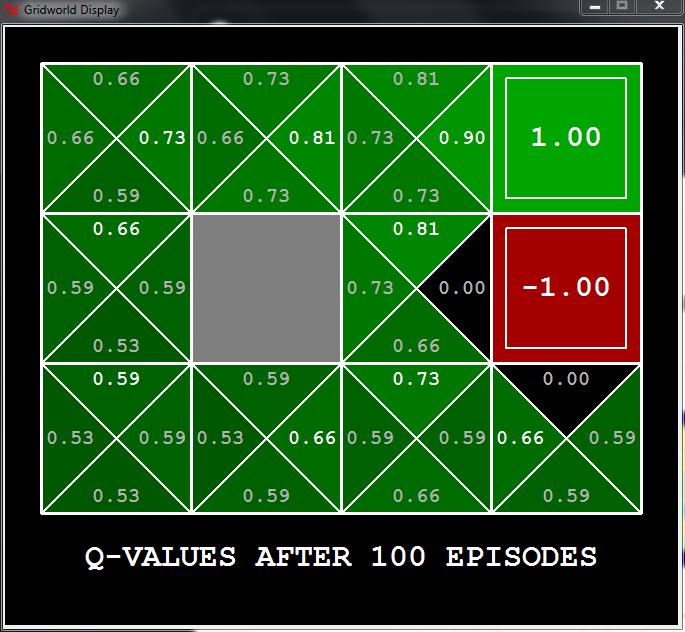
\includegraphics[scale=0.5]{image_3}
	\caption{Interfaz del dominio GridWorld cuando \textit{epsilon} es igual a 1.}
	\label{image_3}
\end{figure}

% Pregunta 8
{ \question Establece en el constructor de la clase \textit{QLearningAgent} el valor de la variable \textit{epsilon} a 0,05. Ejecuta nuevamente con: \textit{python gridworld.py -a q -k 100 -n 0}. ¿Qué sucede?
}

Si consideramos que un episodio termina si se gana (obtenemos un valor de recompensa positivo) o se pierde (obtenemos un a valor de recompensa negativo), decimos que se gana si el agente alcanza el objetivo, la celda etiquetada con un 1, en el estado TERMINAL\_STATE. Por el contrario decimos que se pierde si el agente no alcanza la celda etiquetada con un 1, alcanza la celda etiquetada con un -1 en el estado TERMINAL\_STATE. En ese caso, cuando \textit{epsilon} es igual a 0,05 (ver Figura \ref{image_4}), se logra llegar más veces a la celda etiquetada con un 1, es decir, existen más episodios donde se gana que donde se pierde. Por el contrario cuando \textit{epsilon} es igual a 1, se logra llegar más veces a la celda etiquetada con un -1, es decir, existen más episodios donde se pierde que donde se gana. 

%Concretamente para cada episodio se devuelve el valor de la política óptima, este valor será positivo si hemos ganado, y negativo si hemos perdido, y al final de la ejecución, después de realizar todos los movimientos, se devuelve el valor: \textit{AVERAGE RETURNS FROM START STATE} que es el promedio de todos ellos. Con este valor podemos saber si después de todos los episodios hemos conseguido ganar o perder más veces, consecuentemente si hemos ganado o hemos perdido. Vemos a continuación este valor cuando la variable \textit{epsilon} es igual a 0,05 y cuando es igual a 1.

Cuando \textit{epsilon} es igual a 0,05:
\begin{itemize}
	\item EPISODE 100 COMPLETE: RETURN WAS 0.59049
	\item AVERAGE RETURNS FROM START STATE: 0.530784257974
\end{itemize}

Cuando \textit{epsilon} es igual a 1:
\begin{itemize}
	\item EPISODE 100 COMPLETE: RETURN WAS 0.0119725151826
	\item AVERAGE RETURNS FROM START STATE: -0.079260284124
\end{itemize}	

Comprobamos que cuando \textit{epsilon} es igual a 0,05 ganamos: 0.530784257974 $>= 0$; y cuando \textit{epsilon} es igual a 1 perdemos: -0.079260284124 $<=$ 0.

\begin{figure}[h]
	\centering
	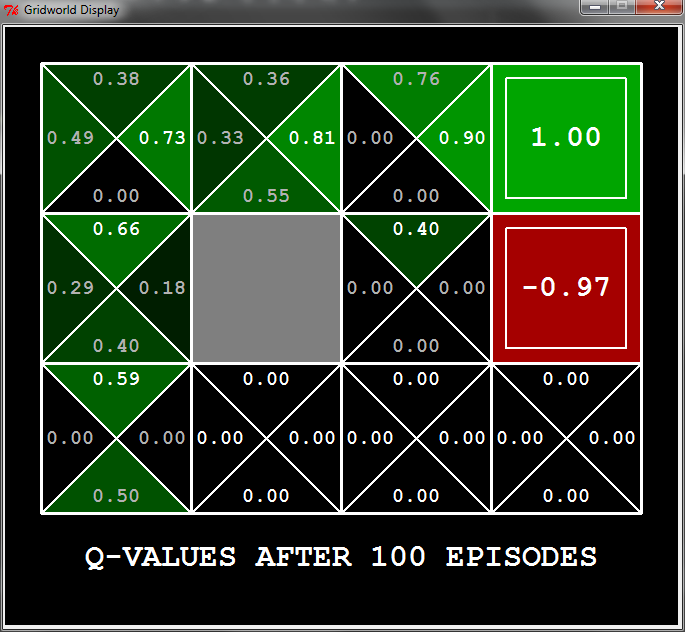
\includegraphics[scale=0.5]{image_4}
	\caption{Interfaz del dominio GridWorld cuando \textit{epsilon} es igual a 0,05.}
	\label{image_4}
\end{figure}

% Pregunta 9
{ \question Después de la ejecución anterior, abrir el fichero \textit{qtable.txt}. ¿Qué contiene?}

El fichero \textit{qtable.txt} contiene los valores de $Q(s,a)$ después de todas las actualizaciones en todos los episodios. Podemos ver el contenido del fichero fichero \textit{qtable.txt} a continuación:

\renewcommand{\tablename}{Tabla}

\begin{table}[h]
	\centering
	\begin{tabular}{|c|c|c|c|c|}
		\hline
		0.59049        & 0.119569809907 & 0.0            & 0.0            & 0.0   \\ \hline
		0.0            & 0.0            & 0.0            & 0.398575844342 & 0.0   \\ \hline
		0.0            & 0.0            & 0.0            & 0.0            & 0.0   \\ \hline
		0.0            & 0.0            & 0.0            & 0.0            & 0.0   \\ \hline
		0.6561         & 0.153677329102 & 0.0            & 0.4428675      & 0.0   \\ \hline
		0.0            & 0.0            & 0.0            & 0.0            & 0.0   \\ \hline
		0.568245849609 & 0.0            & 0.0            & 0.0            & 0.0   \\ \hline
		0.0            & 0.0            & 0.0            & 0.0            & -0.75 \\ \hline
		0.32805        & 0.729          & 0.295245       & 0.327896389246 & 0.0   \\ \hline
		0.0            & 0.81           & 0.364499433769 & 0.0            & 0.0   \\ \hline
		0.0            & 0.9            & 0.148078125    & 0.0            & 0.0   \\ \hline
		0.0            & 0.0            & 0.0            & 0.0            & 1.0   \\ \hline
	\end{tabular}
	\caption{Contenido del fichero \textit{qtable.txt}.}
	\label{table_2}
\end{table}

\end{questions}

\section*{Ejercicio 2}

En el ejercicio anterior, siempre que el agente decidía moverse hacia una dirección se movía en esa dirección con probabilidad 1. Es decir, se trataba de un MDP determinista. Ahora vamos a crear un MDP estocástico.

\begin{questions}

% Pregunta 1
{ \question Ejecuta y juega un par de partidas con el agente manual: \textit{python gridworld.py -m -n 0.3}. ¿Qué sucede? ¿Crees que el agente \textit{QLearningAgent} será capaz de aprender en este nuevo escenario?
}

% Pregunta 2
{ \question Reiniciar los valores de la tabla Q del fichero \textit{qtable.txt}. Para ello ejecutar desde el terminal: \\ \textit{cp qtable.ini.txt qtable.txt}.
}

% Pregunta 3
{ \question Ejecutar el agente \textit{QLearningAgent}: \textit{python gridworld.py -a q -k 100 -n 0.3}.}

\begin{figure}[h]
	\centering
	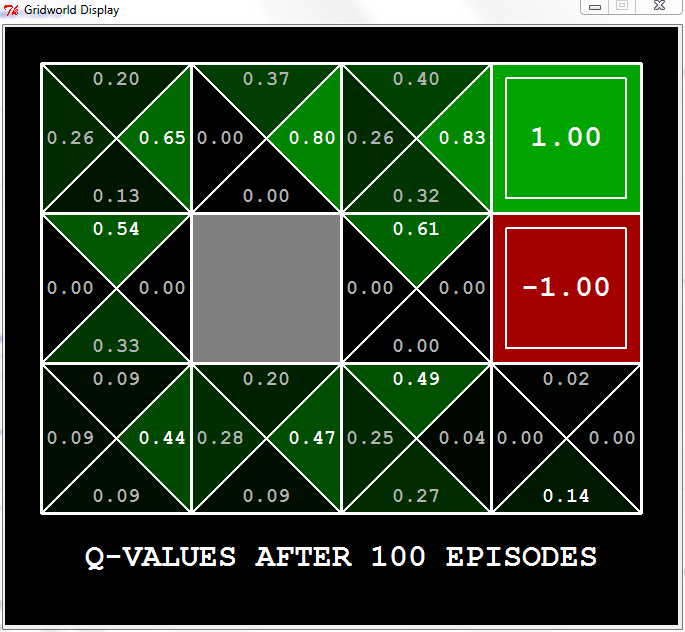
\includegraphics[scale=0.5]{image_5}
	\caption{Interfaz del dominio GridWorld.}
	\label{image_5}
\end{figure}

% Pregunta 4
{ \question Tras unas cuantos episodios, ¿se genera la política óptima? Y si se genera, ¿se tarda más o menos que en el caso determinista?
}

\end{questions}

\end{document}
